Es una forma sencilla de calcular un interés. Suele aplicarse a préstamos para automóviles o préstamos a corto plazo, aunque algunas hipotecas utilizan este método de cálculo. También es el tipo de interés que los bancos pagan a los clientes por sus cuentas de ahorro.

\textbf{Variables}

\begin{itemize}
  \item \textbf{P}: \textit{Principal}. Monto inicial.
  \item \textbf{r}: \textit{Interest rate}. Tasa de interés.
  \item \textbf{n}: \textit{Number of periods}. Número de periodos (diario, semanal, mensual, trimestral, etc) transcurridos respecto al inicio de la entrada en vigor de los intereses.
  \item \textbf{A}: \textit{Amount}. Monto final total.
\end{itemize}

Lo primero es definir un cálculo para obtener el interés. La cual se muestra abajo.

\[
  rP
\]

A esto hay que sumar el monto inicial. Se obtiene lo siguinte:
\[
  A = P + rP
\]

Esto funciona para un periodo, ejemplo un año. Sin embargo, si se quiere obtener el valor para varios periodos, ejemplo dos años, hay que sumar el interés extra.

\[
  A = P + rP + rP
\]

Si se quiere un tercer periodo:

\[
  A = P + rP + rP + rP
\]

De esto se deduce que el interés se calcula con el mismo procedimiento durante múltiples periodos. De lo anterior, se puede reducir la fórmula de la siguiente manera:

\[
  A = P + nrP
\]

Donde $n$ es el numero de periodos. Factorizando $P$ en la expresión se obtiene la siguiente ecuación:

\begin{listequbox}
  {A = P(1 + nr)}{equintsimple}{Interés simple}
\end{listequbox}

Para ilustrar la forma en que crece el interés simple se utilizará el siguiente ejemplo: se efectua un
préstamo de \$100 a una tasa de interés del 10\% durante un periodo de 5 años.

\begin{table}[H]
  \center
  \caption{Evolución interés simple}\label{tabintsimple}
  \begin{tabular}{|c|c|}
    \hline
    \textbf{n} & \textbf{Monto total} \\
    \hline
    0 & 100 \\
    \hline
    1 & 110 \\
    \hline
    2 & 120 \\
    \hline
    3 & 130 \\
    \hline
    4 & 140 \\
    \hline
    5 & 150 \\
    \hline
  \end{tabular}
\end{table}

Se puede observar en la tabla \ref{tabintsimple} que el monto total aumenta de forma constante conforme pasa el tiempo y transcurren los periodos. Esto se debe a que solo se toma en cuenta para los intereses el monto incial, lo que resulta en un crecimiento lineal.

La siguiente gráfica ilustra el aumento del monto total conforme pasa el tiempo.

\begin{grafica}
\center
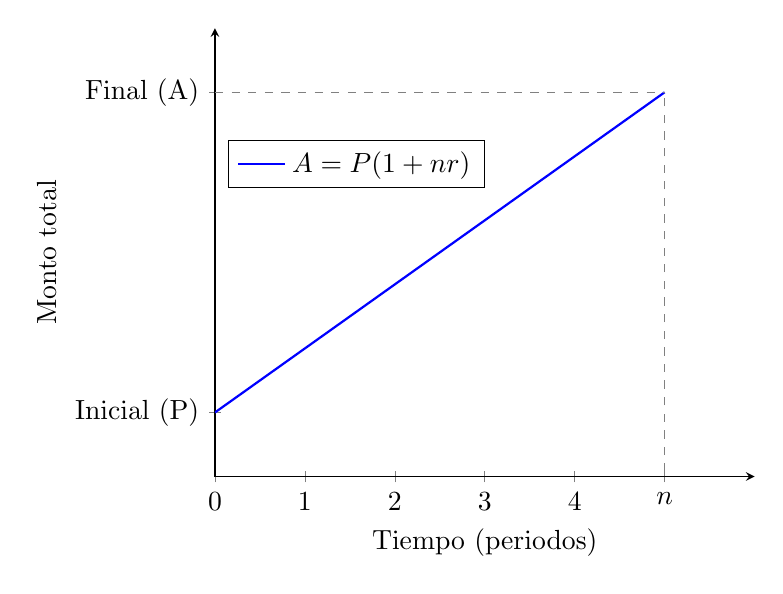
\begin{tikzpicture}
  \begin{axis}[
    xmin=0,xmax=6,
    xtick={0,1,2,3,4,5},xticklabels={0,1,2,3,4,$n$},
    ymin=90,ymax=160,
    ytick={100,150},yticklabels={\text{Inicial (P)},\text{Final (A)}},
    xlabel={\text{Tiempo (periodos)}},
    ylabel={\text{Monto total}},
    legend style={at={(0.5,0.75)}},
    axis lines=left
    ]
    \addplot[color=blue,domain=0:5,thick]{100*(1+(x*0.1))};
    \addlegendentry{$A = P(1 + nr)$}

    \draw[black!50,dashed] (axis cs:5,0) -- (axis cs:5,150);
    \draw[black!50,dashed] (axis cs:0,150) -- (axis cs:5,150);
  \end{axis}
\end{tikzpicture}
\caption{Crecimiento interés simple}
\end{grafica}
